
\documentclass[letterpaper,hide notes,xcolor={table,svgnames},pdftex,10pt]{beamer}
\def\showexamples{t}

\usecolortheme{crane}
\setbeamertemplate{navigation symbols}{}

\usetheme{MyPittsburgh}
\usepackage{hyperref}
\usepackage{graphicx,xspace}
\usepackage[normalem]{ulem}
\usepackage{multicol}
\usepackage{amsmath,amssymb,amsthm,graphicx,xspace}
\newcommand\SF[1]{$\bigstar$\footnote{SF: #1}}

\usepackage[sfdefault,lf]{carlito}
\usepackage[T1]{fontenc}
\usepackage[scaled]{beramono}
\usepackage{tikzpagenodes}
\newcommand{\Rplus}{\protect\hspace{-.1em}\protect\raisebox{.35ex}{\small{\small\textbf{+}}}}
\newcommand{\Cpp}{\mbox{C\Rplus\Rplus}\xspace}

\newcounter{tmpnumSlide}
\newcounter{tmpnumNote}

\newcommand\mnote[1]{%
	\addtocounter{tmpnumSlide}{1}
	\ifdefined\showcues {~\tiny\fbox{\arabic{tmpnumSlide}}}\fi
	\note{\setlength{\parskip}{1ex}\addtocounter{tmpnumNote}{1}\textbf{\Large \arabic{tmpnumNote}:} {#1\par}}}

\newcommand\mmnote[1]{\note{\setlength{\parskip}{1ex}#1\par}}


\newcommand\mquestion[2]{{~\color{red}\fbox{?}}\note{\setlength{\parskip}{1ex}\par{\Large \textbf{?}} #1} \note{\setlength{\parskip}{1ex}\par{\Large \textbf{A}} #2\par}\ifdefined \presentationonly \pause \fi}

\newcommand\blackboard[1]{%
	\ifdefined   \showblackboard
		{#1}
	\else {\begin{center} \fbox{\colorbox{blue!30}{%
						\begin{minipage}{.95\linewidth}%
							\hspace{\stretch{1}} Some space intentionally left blank; done at the blackboard.%
						\end{minipage}}}\end{center}}%
	\fi%
}

\usepackage{listings}
\lstset{%
	keywordstyle=\bfseries,
	aboveskip=15pt,
	belowskip=15pt,
	captionpos=b,
	identifierstyle=\ttfamily,
	frame=lines,
	numbers=left, basicstyle=\scriptsize, numberstyle=\tiny, stepnumber=0, numbersep=2pt}

\usepackage{siunitx}
\newcommand\sius[1]{\num[group-separator = {,}]{#1}\si{\micro\second}}
\newcommand\sims[1]{\num[group-separator = {,}]{#1}\si{\milli\second}}
\newcommand\sins[1]{\num[group-separator = {,}]{#1}\si{\nano\second}}
\sisetup{group-separator = {,}, group-digits = true}

%% -------------------- tikz --------------------
\usepackage{tikz}
\usetikzlibrary{positioning}
\usetikzlibrary{arrows,backgrounds,automata,decorations.shapes,decorations.pathmorphing,decorations.markings,decorations.text}

\tikzstyle{place}=[circle,draw=blue!50,fill=blue!20,thick, inner sep=0pt,minimum size=6mm]
\tikzstyle{transition}=[rectangle,draw=black!50,fill=black!20,thick, inner sep=0pt,minimum size=4mm]

\tikzstyle{block}=[rectangle,draw=black, thick, inner sep=5pt]
\tikzstyle{bullet}=[circle,draw=black, fill=black, thin, inner sep=2pt]

\tikzstyle{pre}=[<-,shorten <=1pt,>=stealth',semithick]
\tikzstyle{post}=[->,shorten >=1pt,>=stealth',semithick]
\tikzstyle{bi}=[<->,shorten >=1pt,shorten <=1pt, >=stealth',semithick]

\tikzstyle{mut}=[-,>=stealth',semithick]

\tikzstyle{treereset}=[dashed,->, shorten >=1pt,>=stealth',thin]

\usepackage{ifmtarg}
\usepackage{xifthen}
\makeatletter
% new counter to now which frame it is within the sequence
\newcounter{multiframecounter}
% initialize buffer for previously used frame title
\gdef\lastframetitle{\textit{undefined}}
% new environment for a multi-frame
\newenvironment{multiframe}[1][]{%
	\ifthenelse{\isempty{#1}}{%
		% if no frame title was set via optional parameter,
		% only increase sequence counter by 1
		\addtocounter{multiframecounter}{1}%
	}{%
		% new frame title has been provided, thus
		% reset sequence counter to 1 and buffer frame title for later use
		\setcounter{multiframecounter}{1}%
		\gdef\lastframetitle{#1}%
	}%
	% start conventional frame environment and
	% automatically set frame title followed by sequence counter
	\begin{frame}%
		\frametitle{\lastframetitle~{\normalfont(\arabic{multiframecounter})}}%
		}{%
	\end{frame}%
}
\makeatother

\makeatletter
\newdimen\tu@tmpa%
\newdimen\ydiffl%
\newdimen\xdiffl%
\newcommand\ydiff[2]{%
	\coordinate (tmpnamea) at (#1);%
	\coordinate (tmpnameb) at (#2);%
	\pgfextracty{\tu@tmpa}{\pgfpointanchor{tmpnamea}{center}}%
	\pgfextracty{\ydiffl}{\pgfpointanchor{tmpnameb}{center}}%
	\advance\ydiffl by -\tu@tmpa%
}
\newcommand\xdiff[2]{%
	\coordinate (tmpnamea) at (#1);%
	\coordinate (tmpnameb) at (#2);%
	\pgfextractx{\tu@tmpa}{\pgfpointanchor{tmpnamea}{center}}%
	\pgfextractx{\xdiffl}{\pgfpointanchor{tmpnameb}{center}}%
	\advance\xdiffl by -\tu@tmpa%
}
\makeatother
\newcommand{\copyrightbox}[3][r]{%
	\begin{tikzpicture}%
		\node[inner sep=0pt,minimum size=2em](ciimage){#2};
		\usefont{OT1}{phv}{n}{n}\fontsize{4}{4}\selectfont
		\ydiff{ciimage.south}{ciimage.north}
		\xdiff{ciimage.west}{ciimage.east}
		\ifthenelse{\equal{#1}{r}}{%
			\node[inner sep=0pt,right=1ex of ciimage.south east,anchor=north west,rotate=90]%
			{\raggedleft\color{black!50}\parbox{\the\ydiffl}{\raggedright{}#3}};%
		}{%
			\ifthenelse{\equal{#1}{l}}{%
				\node[inner sep=0pt,right=1ex of ciimage.south west,anchor=south west,rotate=90]%
				{\raggedleft\color{black!50}\parbox{\the\ydiffl}{\raggedright{}#3}};%
			}{%
				\node[inner sep=0pt,below=1ex of ciimage.south west,anchor=north west]%
				{\raggedleft\color{black!50}\parbox{\the\xdiffl}{\raggedright{}#3}};%
			}
		}
	\end{tikzpicture}
}


%% --------------------

%\usepackage[excludeor]{everyhook}
%\PushPreHook{par}{\setbox0=\lastbox\llap{MUH}}\box0}

%\vspace*{\stretch{1}

%\setbox0=\lastbox \llap{\textbullet\enskip}\box0}

\setlength{\parskip}{\fill}

\newcommand\noskips{\setlength{\parskip}{1ex}}
\newcommand\doskips{\setlength{\parskip}{\fill}}

\newcommand\xx{\par\vspace*{\stretch{1}}\par}
\newcommand\xxs{\par\vspace*{2ex}\par}
\newcommand\tuple[1]{\langle #1 \rangle}
\newcommand\code[1]{{\sf \footnotesize #1}}
\newcommand\ex[1]{\uline{Example:} \ifdefined \presentationonly \pause \fi
	\ifdefined\showexamples#1\xspace\else{\uline{\hspace*{2cm}}}\fi}

\newcommand\ceil[1]{\lceil #1 \rceil}


\AtBeginSection[]
{
	\begin{frame}
		\frametitle{Outline}
		\tableofcontents[currentsection]
	\end{frame}
}



\pgfdeclarelayer{edgelayer}
\pgfdeclarelayer{nodelayer}
\pgfsetlayers{edgelayer,nodelayer,main}

\tikzstyle{none}=[inner sep=0pt]
\tikzstyle{rn}=[circle,fill=Red,draw=Black,line width=0.8 pt]
\tikzstyle{gn}=[circle,fill=Lime,draw=Black,line width=0.8 pt]
\tikzstyle{yn}=[circle,fill=Yellow,draw=Black,line width=0.8 pt]
\tikzstyle{empty}=[circle,fill=White,draw=Black]
\tikzstyle{bw} = [rectangle, draw, fill=blue!20,
text width=4em, text centered, rounded corners, minimum height=2em]

\newcommand{\CcNote}[1]{% longname
	This work is licensed under the \textit{Creative Commons #1 3.0 License}.%
}
\newcommand{\CcImageBy}[1]{%
	\includegraphics[scale=#1]{creative_commons/cc_by_30.pdf}%
}
\newcommand{\CcImageSa}[1]{%
	\includegraphics[scale=#1]{creative_commons/cc_sa_30.pdf}%
}
\newcommand{\CcImageNc}[1]{%
	\includegraphics[scale=#1]{creative_commons/cc_nc_30.pdf}%
}
\newcommand{\CcGroupBySa}[2]{% zoom, gap
	\CcImageBy{#1}\hspace*{#2}\CcImageNc{#1}\hspace*{#2}\CcImageSa{#1}%
}
\newcommand{\CcLongnameByNcSa}{Attribution-NonCommercial-ShareAlike}

\newenvironment{changemargin}[1]{% 
	\begin{list}{}{% 
		\setlength{\topsep}{0pt}% 
		\setlength{\leftmargin}{#1}% 
		\setlength{\rightmargin}{1em}
		\setlength{\listparindent}{\parindent}% 
		\setlength{\itemindent}{\parindent}% 
		      \setlength{\parsep}{\parskip}% 
		      }% 
		\item[]}{\end{list}}




\title{Lecture 11 --- Virtual Memory II }

\author{Jeff Zarnett \\ \small \texttt{jzarnett@uwaterloo.ca}}
\institute{Department of Electrical and Computer Engineering \\
  University of Waterloo}
\date{\today}


\begin{document}

\begin{frame}
  \titlepage

 \end{frame}

\begin{frame}
\frametitle{Memory-Mapped Files}

Remember memory-mapped files for IPC? Let's talk about how it works.

Basic premise: disk blocks mapped to main memory.

First access is a page fault; subsequent accesses are reads/writes.

\end{frame}

\begin{frame}
\frametitle{Table For One Please}

In the one-process scenario, we don't have to synchronize changes.

The memory-mapped file can be in the virtual address space for two different processes.

But we only fetch a block if we must, so synchronization is explicit.

\end{frame}

\begin{frame}
\frametitle{Take Me There}

Memory-mapped I/O -- to communicate with a HW device, an area that looks like main memory is really I/O device memory.

This simplifies some operations!

Kind of like how UNIX treats everything as a file...

\end{frame}

\begin{frame}
\frametitle{Port Mapped}

This contrasts with the older-style \alert{port-mapped} I/O

There are different CPU instructions and separate registers used to communicate with the device. 

\begin{center}
	
\includegraphics[width=0.4\textwidth]{images/translator.jpg}
\end{center}

It's not that this does not work, but it's just more difficult to work with.



\end{frame}


\begin{frame}
\frametitle{Allocation of Frames}

In a simple system with $n$ frames free in the system, demand page all of them. 



\begin{center}
	
\includegraphics[width=0.3\textwidth]{images/pages-elsewhere.jpg}
\end{center}

Initially, all frames are empty, and as needed, pages are read into those frames. 

 \end{frame}


\begin{frame}
\frametitle{Allocation of Frames}

Once all $n$ frames are filled with pages, page $n+1$ must replace a page already in a frame (because there is no more space). 

When a process terminates, all its frames are marked as free. In theory, one process could fill all the frames in the system. 

\begin{center}
	
\includegraphics[width=0.3\textwidth]{images/allmine.jpg}
\end{center}

This is as simple as it can be; from there we can build on it.


\end{frame}

\begin{frame}
\frametitle{Make a Reservation}

We might reserve a few pages to be free at all times for performance reasons

\begin{center}
	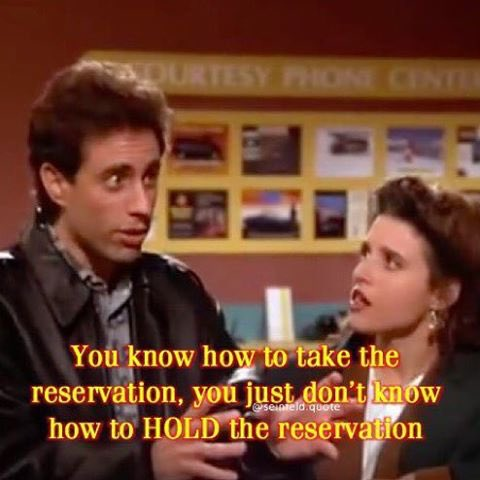
\includegraphics[width=0.5\textwidth]{images/reservation.jpg}
\end{center}

\end{frame}

\begin{frame}
\frametitle{Make a Reservation}

When we want to move a page into a frame, if all of the frames are full, we select a victim and write that victim out to disk if necessary. 

If we keep a few frames free, the newly-read page can be read into one of the free frames, and we can write the old page out to disk at a convenient time. 

The read does not need to wait for the write.

\end{frame}

\begin{frame}
\frametitle{How Many Frames?}

We might want to allocate different numbers of frames to different processes.

We are constrained in the number of pages we can allocate. 

The maximum number of frames a process could have is the maximum number of frames in the system (obviously), but the minimum is more interesting.


\end{frame}

\begin{frame}
\frametitle{Minimum Frames}

The motivation behind a minimum number of frames is ostensibly performance. 

More frames is usually better!

But what determines the minimum?

\end{frame}

\begin{frame}
\frametitle{Minimum Frames}

The absolute minimum number of frames is determined by the architecture. 

\begin{center}
	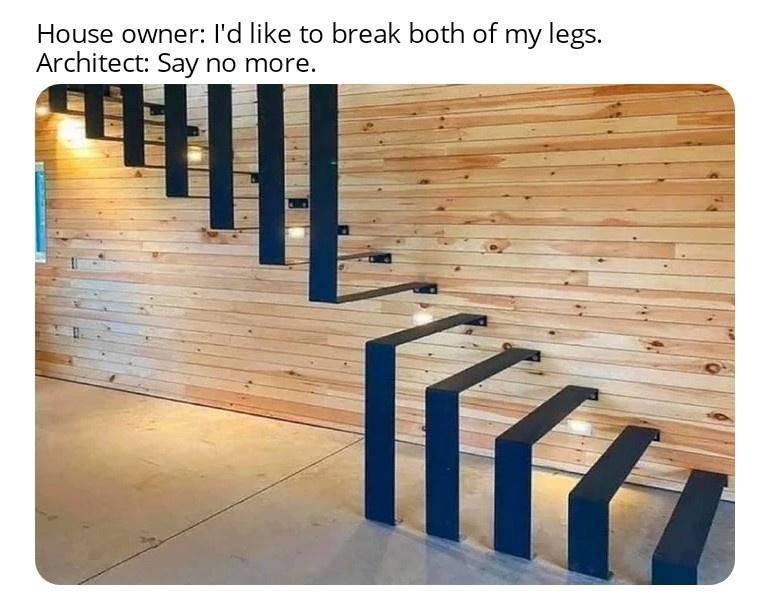
\includegraphics[width=0.75\textwidth]{images/architecture.jpg}
\end{center}

\end{frame}

\begin{frame}
\frametitle{Minimum Frames}



Imagine a machine where a memory reference instruction may contain one memory address.

In the worst case, the instruction and the address are in different pages, so we will need two frames to be able to complete this instruction.

If the max frames for this process were 1, the instruction could never complete.

\end{frame}


\begin{frame}
\frametitle{I'm Still Using That!}

We might need to lock pages in memory for, perhaps, an I/O operation.

For DMA: Lock, transfer, unlock.

Maybe we can avoid it by never transferring directly to/from user memory...\\
\quad Always use kernel buffers instead.

\end{frame}

\begin{frame}
\frametitle{Allocation Strategies}

Assuming we do not allocate every process the minimum or maximum, there are a few allocation algorithms we might follow. 

We already got a glimpse at this when we talked about local vs. global cache replacement.

If there are $m$ frames in the system and the operating system reserves $k$ of them for its own use, there are $m-k$ frames available for processes.

\end{frame}

\begin{frame}
\frametitle{Equal Allocation}

If there are $n$ processes, each process gets $(m-k)/n$ frames. 

If this division produces a remainder, the leftover frames can be kept as a pool of free frames for performance purposes as above. 

But: why does a text editor get the same amount of frames as a web browser?

And the same amount of frames as a game (VERY demanding on memory)?


\end{frame}

\begin{frame}
\frametitle{Proportional Allocation}

Each process should get a share of the frames based on its needs. 

Let the virtual memory size of a process $p_{i}$ be defined as $s_{i}$. 

Thus $S = \Sigma s_{i}$. 

Then we allocate $a_{i}$ frames to a process $p_{i}$ according to the formula: 

$a_{i} = s_{i} / S \times (m - k)$.

\end{frame}

\begin{frame}
\frametitle{Proportional Allocation}

This value of $a_{i}$ is only an estimate. 

It may not divide evenly: rounding is required; minimums need to be enforced.

A few of the larger processes may need to have their allocations nudged down.


\end{frame}

\begin{frame}
\frametitle{Proportional Allocation}

Note that with proportional allocation, as with equal allocation, there is no regard given to the priorities of the processes. 

We could modify the $a_{i}$ values according to process priority. 

Priority matters a lot in scheduling... soon...

\end{frame}


\begin{frame}
\frametitle{Thrashing}
This topic was previously introduced, and now we'll come back to it.

The quick definition of thrashing still applies.

Aside from intentionally depriving the system of RAM, how can we get into this state, and how can we get out of it?


\end{frame}

\begin{frame}
\frametitle{Thrashing}

In simple operating systems, the logic that controlled how many processes to run at a time would rely just on the CPU utilization. 

If CPU utilization is low, the CPU needs more work to do! 

\begin{center}
	
\includegraphics[width=0.4\textwidth]{images/backtowork.jpg}
\end{center}

\end{frame}

\begin{frame}
\frametitle{Thrashing}

Assign it more work by starting or bringing more processes into memory. 

The global page replacement policy is used here, so when a process gets a page fault, it takes a frame from another process. 

Under most circumstances, this works just fine.

\end{frame}

\begin{frame}
\frametitle{Downward Spiral}

This situation can run until one process starts to have a lot of page faults. 

This is not unreasonable; a compiler might be finished with reading and parsing the input files and moving to generation of binary code. 

This requires a whole bunch of new instructions pages, plus pages for output. 

When this process does so, it starts taking pages from other processes.

\end{frame}

\begin{frame}
\frametitle{Downward Spiral}

The victim processes need the pages they had, so when they get a turn to run, they too start generating page faults. 

So more and more requests are queued up for memory writes and reads, so the CPU is not very busy. 

Here's the fatal mistake: seeing that the CPU is not very busy, the OS schedules \textbf{more} programs to run.  

\end{frame}

\begin{frame}
\frametitle{The Doom in Thrashing}

A new process getting started will need at least the minimum number of pages. 

These have to come from somewhere, so they will necessarily come from the pages currently belonging to other processes. 

This causes more page faults, more time spent paging, lower CPU utilization...\\
\quad Prompting the OS to start more processes. 
\end{frame}

\begin{frame}
\frametitle{Whiplash!}

No more work is getting done, because the system spends all its time moving pages into and out of memory, thrashing all around, acting like a maniac.

\begin{center}
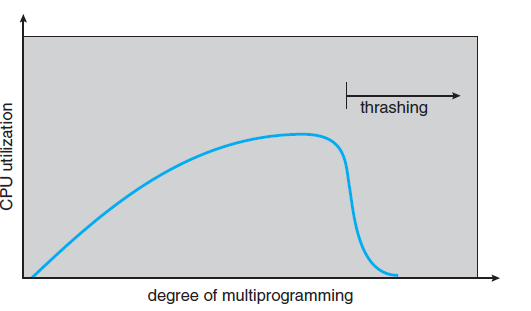
\includegraphics[width=0.75\textwidth]{images/thrashing.png}
\end{center}

\end{frame}

\begin{frame}
\frametitle{Breaking the Spiral}

To increase CPU utilization we need to stop the thrashing...\\
\quad which means we need \textbf{fewer} programs in memory at a time. 

CPU usage alone is not a sufficient indicator of whether more or fewer processes need to be running right now. 

It also matters \textit{why} the CPU utilization is low. Another reason that might cause low CPU usage is, as you may recall, deadlock. 


\end{frame}

\begin{frame}
\frametitle{Local Replacement Instead}

What if we stop using a global replacement policy and instead use local? 

This limits some of the damage;\\
\quad If $P_{1}$ is thrashing, it cannot steal pages from $P_{2}$.\\
\quad We do not get a cascade.

But $P_{2}$ is still affected.

If $P_{1}$ is spending all its time paging to and from disk, any other process that wants to use the disk is going to have to spend more time waiting for the disk.


\end{frame}

\begin{frame}
\frametitle{Starting and Suspending Processes}

Decide whether to start or suspend programs not just based on CPU usage, but also on the number of page faults that occur in a given period of time. 

If there are too many page faults, it indicates we have too much going on. 

That is a reactive solution, however. 

It would be better to be proactive and deal with this before thrashing has started.


\end{frame}

\begin{frame}
\frametitle{More Clairvoyance}

As is typical, a bit of clairvoyance would help here: how many pages is the process going to need and when will it need them? 

Unfortunately, there is no good way to know or to figure this out. So we will have to rely on (educated) guessing.

\end{frame}

\begin{frame}
\frametitle{Making Our Best Guess}

What do we know about process memory accesses? 

They tend to obey the principle of locality, both temporal and spatial.

We could think of different parts of the program as different localities, as if they were areas on a map. And localities may overlap sometimes. 

\end{frame}

\begin{frame}
\frametitle{Making Our Best Guess}

Give a process enough frames for its locality. 

It can operate in this little area without encountering (too many) page faults.


\end{frame}

\begin{frame}
\frametitle{Check Assumptions}

\begin{center}
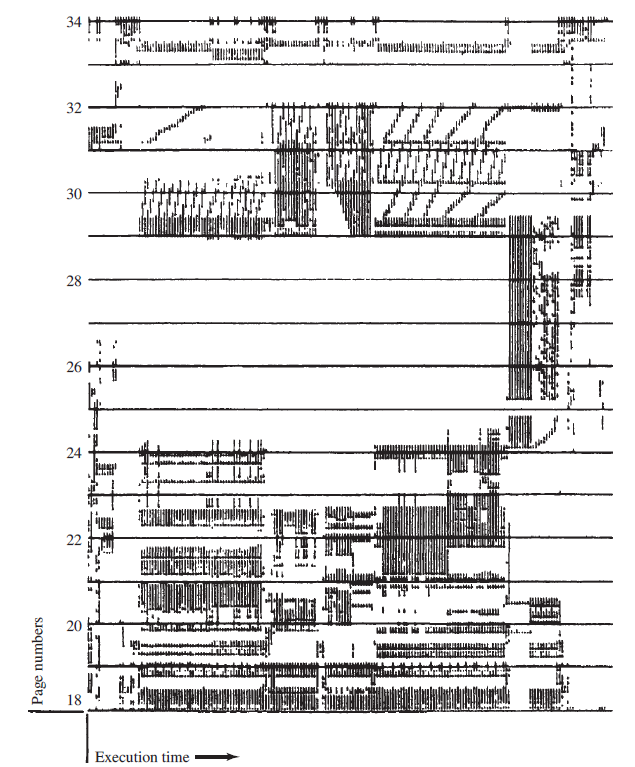
\includegraphics[width=0.55\textwidth]{images/locality.png}
\end{center}


\end{frame}

\begin{frame}
\frametitle{The Working-Set Model}

A potential solution is the working-set model. 

Retain the last $n$ pages in memory as they represent the locale of the program. 

Assuming that most memory accesses are local, the most recent $n$ pages will be the most frequently used.


\end{frame}

\begin{frame}
\frametitle{The Working-Set Model}

In the textbook descriptions, this $n$ is usually called $\Delta$, the working set window. 

Pages that have been recently used are in the working set. 

If a page has not been accessed recently, it will drop out of the working set after $\Delta$ time units since its last reference. 

\end{frame}

\begin{frame}
\frametitle{Working Set Example}

Suppose the window is defined as being ten accesses. 

Any page that was accessed in the last ten requests will then be considered part of the working set. 

If the next ten memory accesses are all in page $k$, then after those further ten accesses, the working set will contain only $k$. 

The size of the working set will change over time; can be from 1 to $\Delta$ pages.

\end{frame}

\begin{frame}
\frametitle{Choosing Delta}

If $\Delta$ is too small, the working set will not encompass the entire locale. 

If it is too large, it will cover multiple locales. 

Underestimating the size of the locale is bad; it will mean more page faults.


Overestimating is also bad; it means fewer processes will be allowed to run.

\end{frame}

\begin{frame}
\frametitle{Sum of the Working Sets}

If the working set of every process is summed up, we will get the total number of frames each process would ``like'' to have. 

If this sum exceeds the $(m-k)$ available frames in the system, at least one process is going to be unhappy.

It does not have as many frames as it will need. 

And like unhappy workers who go on strike, unhappy process start thrashing.


\end{frame}

\begin{frame}
\frametitle{Working Sets}

Once a value of $\Delta$ is determined, the OS will monitor the working set of each process and use that to figure out if the system is currently overloaded. 

If it is, the OS will pick a victim and suspend it to prevent thrashing. 

If the system is underloaded (frame supply exceeds demand), more processes can be started to run.


\end{frame}

\begin{frame}
\frametitle{Working Set}

The page fault rate of a process tends to vary over time. 

At the beginning, there will be a bunch of page faults as the program starts up. 

Then once established in its first locale, the rate will drop. 

When it come time to move to a new locale, the page fault rate rises until the program is ``settled'' in that new locale.


\end{frame}

\begin{frame}
\frametitle{Working Set}

\begin{center}
	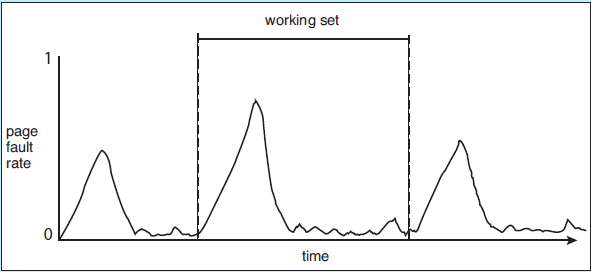
\includegraphics[width=0.75\textwidth]{images/workingset.png}
\end{center}


\end{frame}

\begin{frame}
\frametitle{Working Set Analogy}

Imagine that you have moved to a new city for a co-op term. 

\begin{center}
	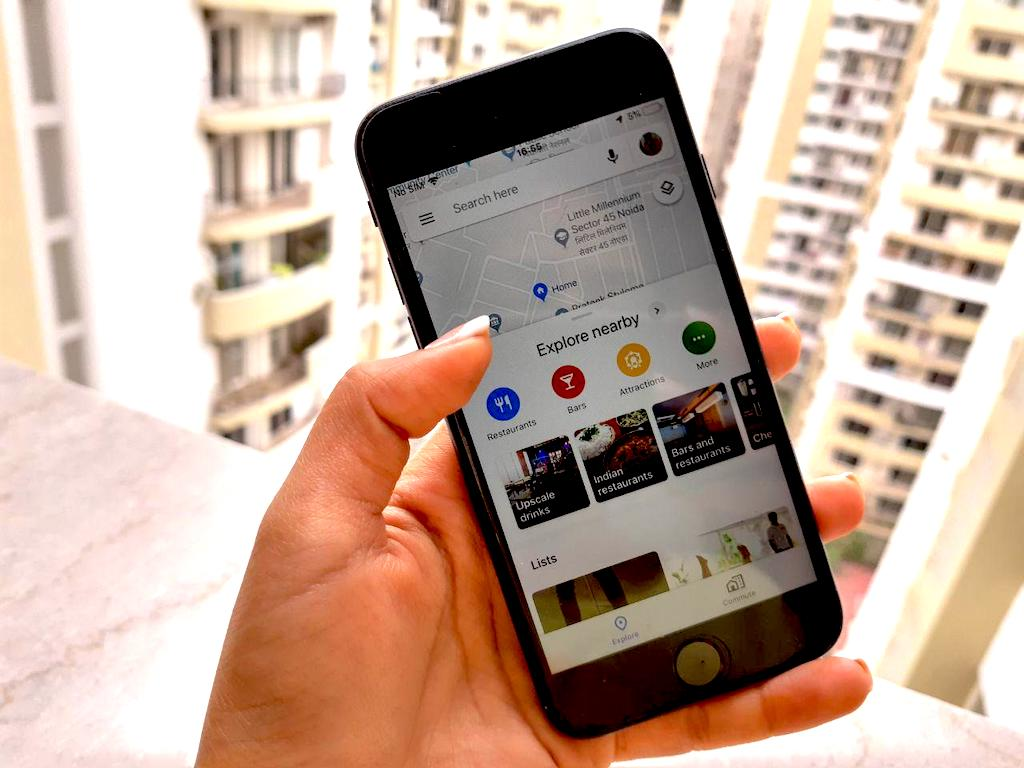
\includegraphics[width=0.75\textwidth]{images/explorenearby.jpg}
\end{center}

\end{frame}

\begin{frame}
\frametitle{Working Set Analogy}
When you have just moved, you will frequently rely on Google Maps to find what you are looking for and how to get there. 

You need to buy groceries, so you ask Google for directions to the nearest grocery store of choice. 

Once you've been there, you know the way so you don't have to ask again. 


\end{frame}

\begin{frame}
\frametitle{Working Set Analogy}

Not knowing where the grocery store is equals a page fault, and asking Google is like asking the operating system to bring in that page from disk. 

Once you know the way to the grocery store, it is part of your working set and you do not have to ask again.


... Until your next co-op term when you move somewhere else.

\end{frame}

\end{document}

